\chapter{Implementation and Evaluation}\label{cha:4_implementation_and_evaluation}
Taking into account the importance of community detection, it is not surprising that many community detection methods have been developed, using tools and techniques from variegated disciplines such as statistical physics, biology, applied mathematics, computer science and sociology \cite{ref-49}. All these methods aim at improving the identification of meaningful communities while keeping as low as possible the computational complexity of the underlying algorithm. Community detection algorithms can differ in two ways: not only the process leading to an estimation of the community structure, but also the nature of the estimated communities themselves \cite{ref-50}. 

For the scope of this thesis, this chapter will discuss the procedure of implementing of the proposed prototypical framework (chapter \ref{cha:3_concept_and_design}) and also explore and evaluate the range and performance capabilities of community detection algorithms in respect to computational complexity and memory space complexity on large scale networks. As Orman et. al in \cite{ref-50} stated that community detection algorithms can differ in two ways, first, algorithms can explore the idea of detecting communities and second, paves the way do discovering the true nature or properties of the detected communities. This chapter (\ref{cha:4_implementation_and_evaluation}) aims to explore the computational complexities at run-time for large-scale networks focusing on blockchain transaction network. At the end of this chapter, an evaluation of the proposed prototypical framework's observation technique is provided based on blockchain network transaction data.

\section{Implementation}
To implement the concept of the framework designed in chapter (\ref{cha:3_concept_and_design}), a certain amount of challenges were faced before the actual implementation could be done. For the scope of the thesis, blockchain transaction data is being used to represent large-scale networks. Each blockchain transaction data has many properties\footnote{Transaction hash, source account hash, transfer amount hash, target account hash, height of the block, age of the block, transactions, contracts attached to the transaction etc.} but for the interest of detecting communities and observing changes afterwards, source account of the transaction, target account of the transaction, amount transferred and the time-stamp, when the transaction has happened is considered in the data-set. \texttt{0x00f41ae83220a4953979fac1dca4433d27439fd0} is an example of a typical hashed account, a transferred amount looks similar to \texttt{2300958728094382741313} and a time stamp is a regular UNIX based time-stamp. So for a single record in the data-set, there are two account address, one transferred amount and a time-stamp.

Before the actual implementation of the proposed framework, there are a few challenges that needed attention. Although every record is time-stamped, to detect community structures in blockchain network the hashed accounts occupies much more memory (RAM) and it limits the power of the community detection algorithms in respect to memory requirement at run-time. Even in high end systems this effects the performance because the whole data-set is loaded into memory at once for community detection. Another issue is the transferred amount, the amount works as a weight of the link between source and target address. As the transferred amount is very big integer, it is not feasible to use this as a weight. 

As a preparation step of the proposed framework, All the hashed addresses in the entire data-set has been mapped to a numeric value. It significantly reduces the memory consumption at run-time leading better performance of the algorithms and the framework as whole. As the memory requirement is lower with numeric data-set, more records of data can be processed with a medium or normal computer system\footnote{Intel(R) Core(TM) i5-3320M CPU @ 2.60GHz and 16 GB of RAM, with 64 bit UNIX Operating System}.  The problem with a very large integer value for the weight (amount) is solved by taking natural logarithm of the actual number and using it as weight. The idea here is to keep a low weight value for the link between source address and target address without compromising the actual importance of the link.

The implementation of the framework has 4 different step done in two different time-stamps. In both the time-stamp, community detection has been done with either infomap, louvain or clauset-newman-moore algorithm. Framework currently supports these three widely used algorithm for community detection. In section (\ref{sec:evaluation}), all of these three community detection algorithm has been evaluated with blockchain data.

At the beginning of the implementation, top $n$ communities are selected form the detected communities. The selection of top $n$ communities is based on the total number of nodes in each community. The community has the highest number of nodes is the largest community. Only the top $n$ largest community is picked up as top $n$ communities. Top $n$ communities are selected because it helps to focus on the communities that are really important. In blockchain data, there could be a numerous number of small communities with a less number of nodes. Picking up top communities removes the idea of picking a small community that has a little or no effect on the entire graph representing a blockchain network.

\begin{figure}[H]
	\centering
	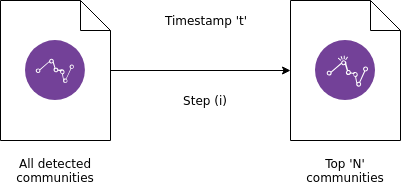
\includegraphics[width=0.5\textwidth]{framework_step_i}
	\caption{Framework: step (i)}
	\label{fig:community}
\end{figure}

In step 2(a), A sub-graph of the data-set from time-stamp $t$ is rendered according to the nodes that are present in the top $n$ communities from step one. The benefit of taking a sub-graph that has been carefully selected from the nodes that are present in top $n$ communities is that only the data that is required to track these top $n$ communities will be present in the sub-graph. A blockchain data-set can carry huge amount of transaction records and trying to use all of the records every time can drastically change the behavior of the community detection algorithms as well as the framework. If all the data is selected, the framework will try to calculate communities for nodes that is not in the target communities, resulting in longer run-time and not to mention more memory consumption.

\begin{figure}[H]
	\centering
	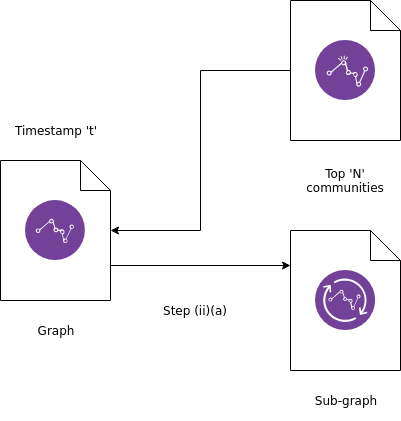
\includegraphics[width=0.5\textwidth]{framework_step_ii_a}
	\caption{Framework: step (ii)(a)}
	\label{fig:community}
\end{figure}

In the next step, two snapshots, the sub-graph from 2(a) and a snapshot of data-set from time-stamp $t+1$ are merged to create a unified snapshot of data-set for the next step. The reason for doing this is to prevent nodes from falling out from the data-set at time-stamp $t+1$. Creating a sub-graph from the data-set at time-stamp $t$ helps to reduce the number of records in the current ($t+1$ snapshot), by  adding all the nodes from time-stamp $t$ helps to keep the previous community structures intact so that with the current time-stamp, the change in the community structures are visible.

\begin{figure}[H]
	\centering
	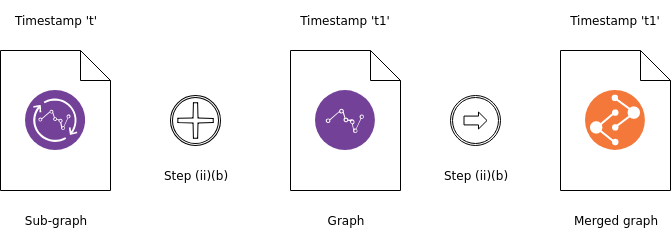
\includegraphics[width=0.7\textwidth]{framework_step_ii_b}
	\caption{Framework: step (ii)(b)}
	\label{fig:community}
\end{figure}

Next step, repeats step one (i) on merged graph data-set to detect communities and to find out top $n$ communities from step 2(b) using the same algorithm that was used in step one for the data-set in time-stamp $t$. But, the problem is that community can change drastically over a time stamp in a network like blockchain data. As it's known that blockchain transactions are used for asset transfer, one node can just stop accepting or sending assets at the next time stamp. So to observe the change in communities, finding the similar pair of community in time-stamp $t$ and $t+1$ is important.

\begin{figure}[H]
	\centering
	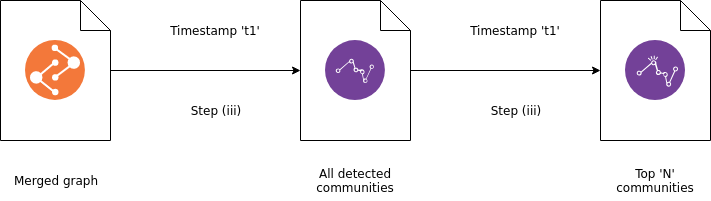
\includegraphics[width=0.7\textwidth]{framework_step_iii}
	\caption{Framework: step (iii)}
	\label{fig:community}
\end{figure}

In the last step of the framework, similarity between community pairs are drawn by the means of similarity measures described in section (\ref{vertexsimilarity}) of this thesis. Similarity measures identifies the similar communities. If top $n$ communities from time-stamp $t$ doesn't have a similar community in top $n$ communities of time-stamp $t+1$, it indicates that the community from time-stamp $t$ has lost nodes and died or became smaller. It also means that some community has been born in time-stamp $t+1$

\begin{figure}[H]
	\centering
	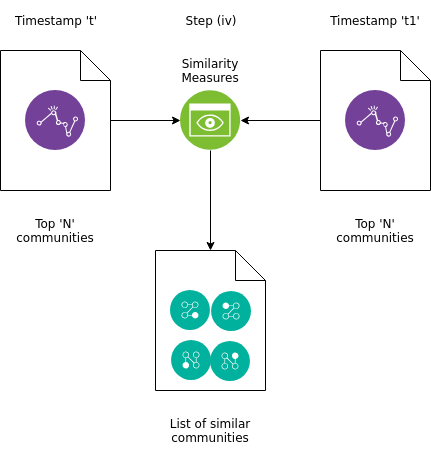
\includegraphics[width=0.5\textwidth]{framework_step_iv}
	\caption{Framework: step (iv)}
	\label{fig:community}
\end{figure}

For the scope of the thesis, implementation of the proposed framework has been done with the help of \texttt{python} programming language. Evaluation results are discussed in the next section (\ref{sec:evaluation}) in respect to run-time and memory consumption.

\section{Evaluation}\label{sec:evaluation}
Over the years different methods have been published and claimed to be the fastest and accurate. But for the scope of this thesis, three most popular and well known algorithms are chosen to test the range of capabilities on run-time complexities and memory requirement. The obvious questions like why these particular algorithms? why not others? will be answered sequentially later in this chapter.

\subsection{Infomap}
%\textit{Infomap} uses map equation (\ref{subsec:map_equation}) from \cite{ref-43}, first introduced in 2009 by Rosvall et al. Infomap represents the community structure through two-level nomenclature based Huffman coding \cite{ref-44}. One level to distinguish communities in the network and the other, to distinguish nodes in a community. In infomap algorithm the problem of finding the best community structure is expressed as minimizing the quantity of information needed to represent some random walk in the network using this nomenclature. With a partition containing few inter-community links, the walker will probably stay longer inside the community, therefore only the second level be needed to describe its path, leading to compact representation. 
%%
Infomap algorithm starts with encoding the network into modules in a way that maximizes the amount of information about the original network. Then it sends the signal to a decoder through a channel with limited capacity. The decoder tries to decode the message and to construct a set of possible candidates for the original graph. The smaller the number of candidates, the more information about the original network has been transferred \cite{ref-49}. This algorithm runs in $\mathcal{O}(E)$, here $E$ is the number of edges. 

The main reason for choosing this algorithm for performance analysis in large-scale networks is its run-time complexity. In \cite{ref-47}, authors stated that this algorithm works in reasonable amount of time for detecting communities in large-scale\footnote{A network with over $1,000,000$ nodes/edges.}\label{foot:large-scale} networks. Memory consumption is also reasonable according to \cite{ref-47}. For the scope of this thesis, this algorithm's performance is being tested against blockchain transaction data to determine community structure in blockchain transactions. to determine the memory usage and run-time of this algorithm for detecting communities in blockchain data in a large network, sample data-sets from \textit{Ethereum} and \textit{Bitcoin} transactions has been used. Data has been analyzed in the same system\footnote{Intel(R) Core(TM) i5-3320M CPU @ 2.60GHz and 16 GB of RAM, with 64 bit UNIX Operating System} the framework has been implemented. 

In Figure (\ref{fig:infomap_runs}) (a) shows the run-time required for infomap to detect community structures. In (a) we can observe that with the growth of the number of nodes the run-time grows but it takes less than a minute to analyze and detect communities in 2.4 Million nodes. In terms of memory, in Figure (b) for the same amount of nodes it took only 5.1 GB of memory. In Figure, (c) and (d), run-time and memory usage reflects in respect to the number of edges. As its seen in these figures, the run-time and memory consumption both goes down on 3rd iteration because of the data-set is more connected. In general, the nodes are more connected and have more links between each other. In terms of communities, Figure (e) and (f) show that it can detect fair amount of communities also. As the blockchain data doesn't follow any pattern or network structure like social media so the data is more sparse than expected. Yet, there are community structures in transaction data. Infomap was able to detect communities in blockchain data-sets proving that community structures exists in blockchain data. To rectify and modify the community detection criteria in large scale data is out of the scope of current chapter. This topic will be introduced in the following chapter. For the scope of the thesis, the main focus was to determine run-time and memory usage for community detection algorithms in bloackcahin transaction data. In respect to run-time and memory usage, infomap algorithm is quite faster and has a reasonably low memory consumption. 
\vfill

% Plot run-time and memory against nodes
\begin{figure}[H]
  \centering
  \begin{minipage}[b]{0.4\textwidth}
    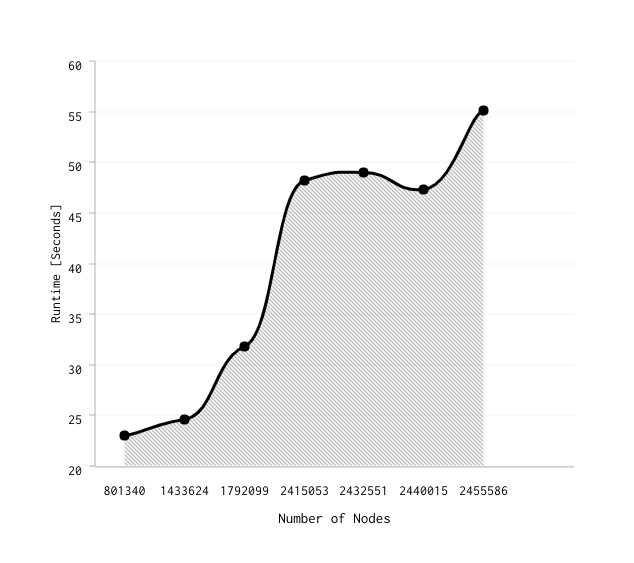
\includegraphics[width=\textwidth]{Infomap-NodesVsRuntime}
    \caption*{(a)}
  \end{minipage}
  %\hfill
  \begin{minipage}[b]{0.4\textwidth}
    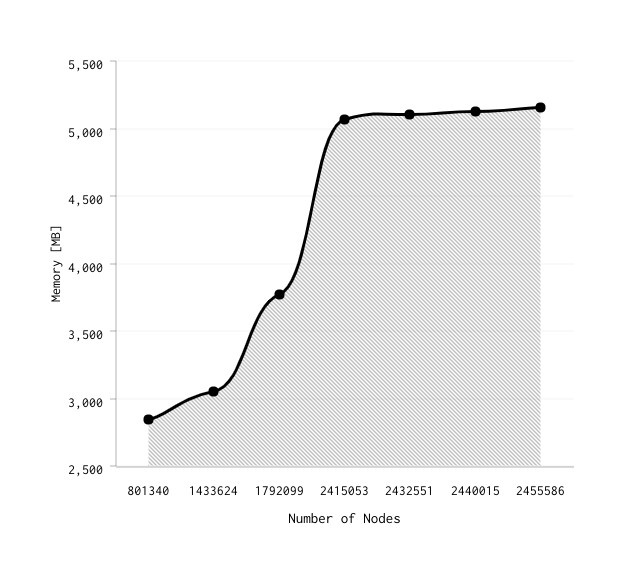
\includegraphics[width=\textwidth]{Infomap-NodesVsMemory}
    \caption*{(b)}
  \end{minipage}
  %hfill
  \begin{minipage}[b]{0.4\textwidth}
    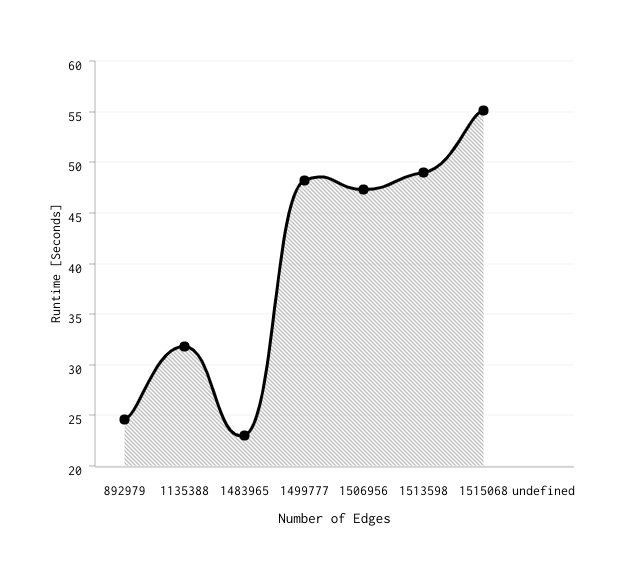
\includegraphics[width=\textwidth]{Infomap-EdgesVsRuntime}
    \caption*{(c)}
  \end{minipage}
  %\hfill
  \begin{minipage}[b]{0.4\textwidth}
    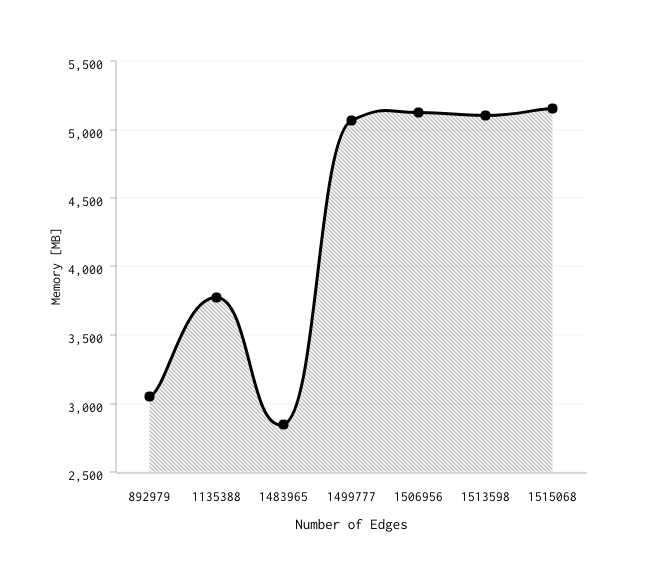
\includegraphics[width=\textwidth]{Infomap-EdgesVsMemory}
    \caption*{(d)}
  \end{minipage}
  %hfill
  \begin{minipage}[b]{0.4\textwidth}
    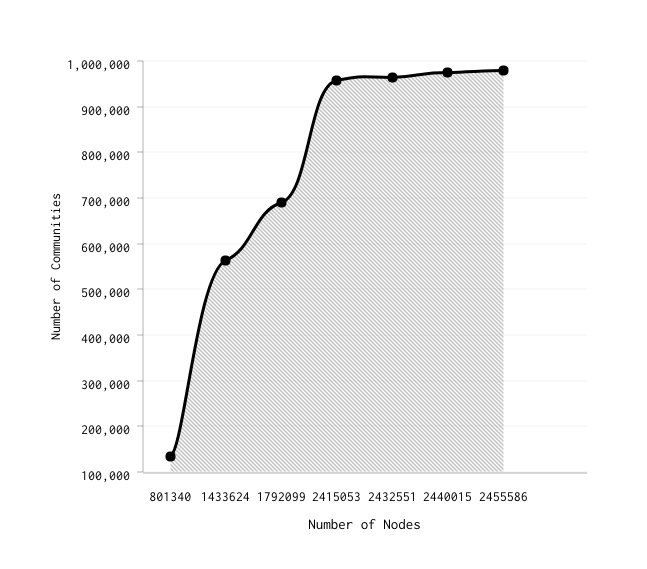
\includegraphics[width=\textwidth]{Infomap-NodesVsCommunities}
    \caption*{(e)}
  \end{minipage}
  %\hfill
  \begin{minipage}[b]{0.4\textwidth}
    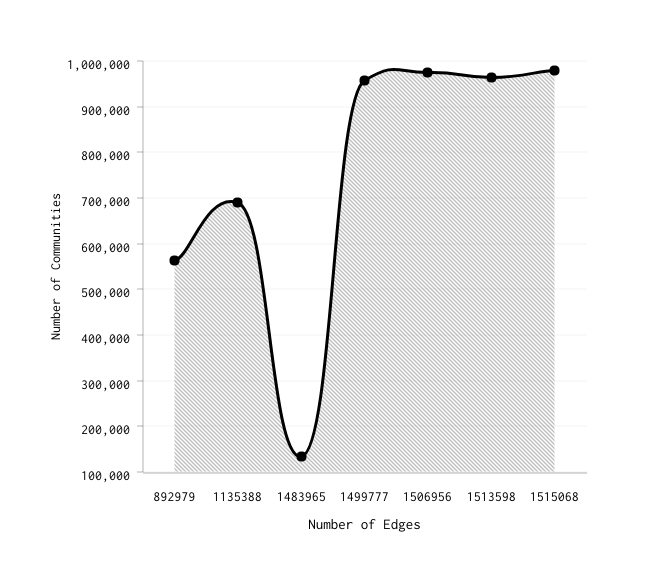
\includegraphics[width=\textwidth]{Infomap-EdgesVsCommunities}
    \caption*{(f)}
  \end{minipage}
  \caption{Infomap algorithm: (a) Run-time against number of nodes (b) Memory usage against number of nodes (c) Run-time against number of edges (d) Memory usage against number of edges (e) Number of communities against number of nodes (f) Number of communities against number of edges}
  \label{fig:infomap_runs}
\end{figure}


\subsection{Louvain}
\textit{Louvain} method (\ref{subsec:generalized_louvain}) is a heuristic method that is based on modularity optimization (\ref{subsec:modularity_maximization}). In \cite{ref-27}, Blondel et al. claimed that louvain method outperforms all other known community detection algorithm in terms of computation time. Moreover, the quality of detected communities is very good, as measured by modularity.

%Louvain algorithm is divided into two phases that are repeated iteratively. Consider a graph representing a network that has $n$ nodes. First, a different community is assigned to each node of the network. So, initially the number of communities are equal to the number of nodes. Then, for each node $i$, the neighbors $j$ of $i$ is evaluated for modularity gain if the node $i$ is removed form it's current community and placing it into the community of $j$. The node $i$ is then placed into the community with maximum gain but only if this gain is positive. If no positive gain is possible, $i$ stays in its original community.This process is applied repeatedly and sequentially for all the nodes until no further improvement can be achieved. In the second phase of the algorithm a new network is constructed whose nodes are now the communities found during the first phase. To do so, the weights of the links between the new nodes are given by the sum of the weight of the links between nodes in the corresponding two communities.
%%
Louvain method is selected for performance analysis in large-scale network because in \cite{ref-27}, authors stated that it outperforms any other community detection algorithm in terms of community detection. This algorithm runs in $\mathcal{O}(N \, log N)$, here $n$ is the number of nodes. For detecting community structures in large-scale blockchain networks, this algorithm can prove to be useful in terms of computation time and memory consumption.

In Figure (\ref{fig:louvain-runs}) (a), shows the run-time required for detecting communities in large scale network. Figure (a) shows the run-time in respect to number of nodes. While the number of nodes increases, the run-time increases too. In Figure (b), the memory usage has been shown in respect to same number of nodes. Louvain method has detected communities in blockchain transaction data in quite reasonable time and with a decent amount of memory usage. Louvian method can detect communities in blockchain data with 2.4 Million nodes in about 700 seconds and the memory usage is about 6.5 GB. In Figure (c) and (d), it shows the run-time and memory consumption of louvain method in respect to number of edges. In 3rd iteration, the run-time and memory usage is lower because the nodes are more closely connected in this graph. For detected community structures, Figure (e) and (f) gives number of detected communities in respect to number of nodes and number of edges. It is noticeable that, for over 1.4 million edges the detected communities by louvain method is nearly 300 only and this is because of the  previously explained issue that this particular graph's nodes are more connected then the other graphs. Louvain method is quite faster and reasonable in memory consumption but with the growing number of nodes the run-time might get higher really quick.

\vfill
\pagebreak

% Plot run-time and memory against nodes
\begin{figure}[H]
  \centering
  \begin{minipage}[b]{0.4\textwidth}
    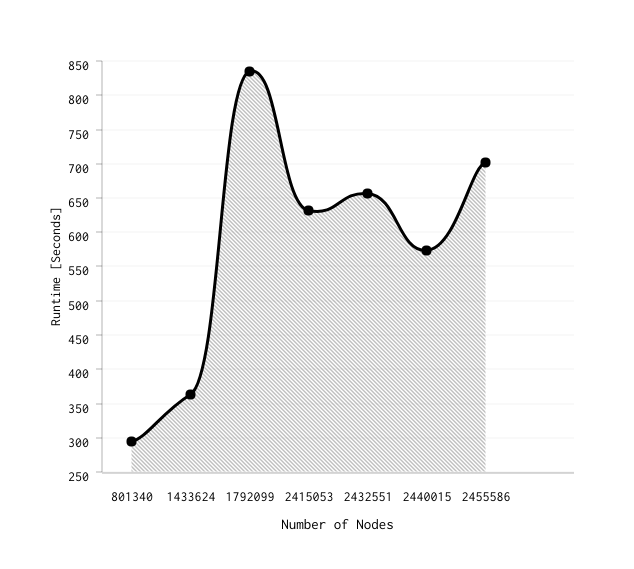
\includegraphics[width=\textwidth]{Louvain-NodesVsRuntime}
    \caption*{(a)}
  \end{minipage}
  %\hfill
  \begin{minipage}[b]{0.4\textwidth}
    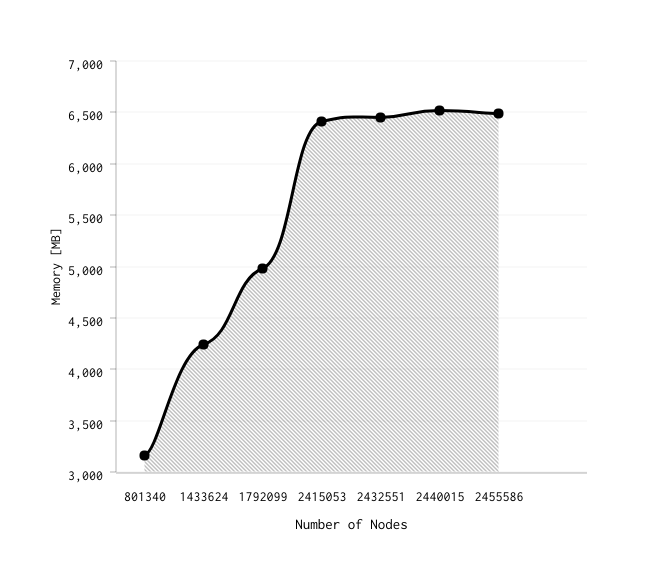
\includegraphics[width=\textwidth]{Louvain-NodesVsMemory}
    \caption*{(b)}
  \end{minipage}
%\end{figure}
%
%% Plot run-time and memory against edges
%\begin{figure}[!tbp]
%  \centering
  \begin{minipage}[b]{0.4\textwidth}
    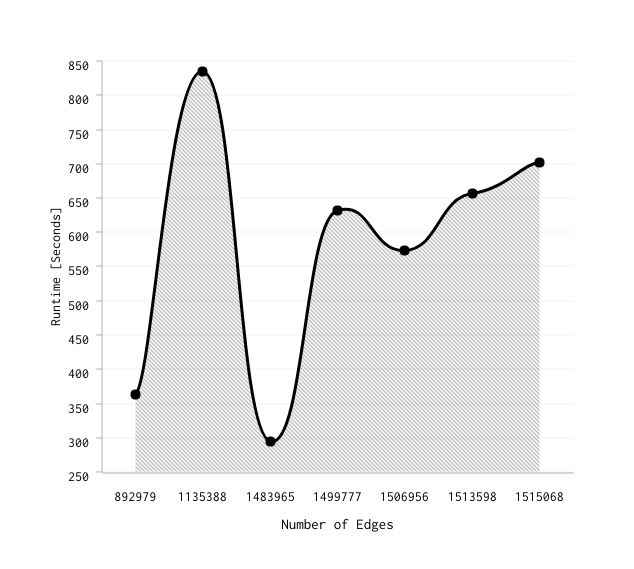
\includegraphics[width=\textwidth]{Louvain-EdgesVsRuntime}
    \caption*{(c)}
  \end{minipage}
  %\hfill
  \begin{minipage}[b]{0.4\textwidth}
    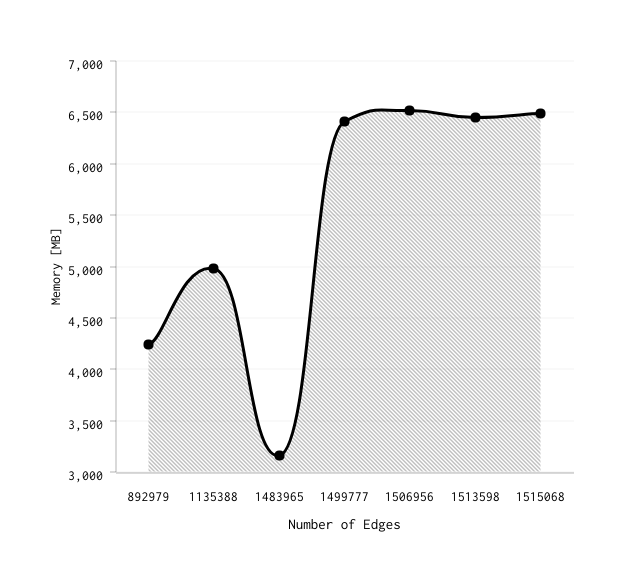
\includegraphics[width=\textwidth]{Louvain-EdgesVsMemory}
    \caption*{(d)}
  \end{minipage}
%\end{figure}
%
%% Plot detected communities
%\begin{figure}[!tbp]
%  \centering
  \begin{minipage}[b]{0.4\textwidth}
    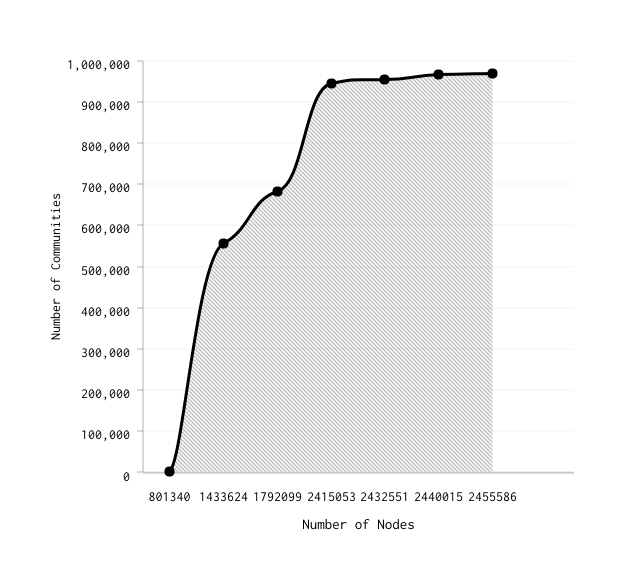
\includegraphics[width=\textwidth]{Louvain-NodesVsCommunities}
    \caption*{(e)}
  \end{minipage}
  %\hfill
  \begin{minipage}[b]{0.4\textwidth}
    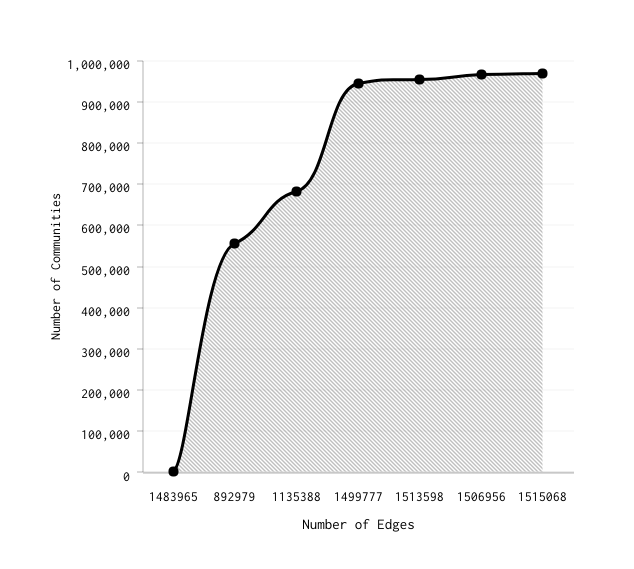
\includegraphics[width=\textwidth]{Louvain-EdgesVsCommunities}
    \caption*{(f)}
  \end{minipage}
  \caption{Louvain method algorithm: (a) run-time against number of nodes (b) usage against number of nodes (c) run-time against number of edges (d) Memory usage against number of edges (e) Number of communities against number of nodes (f) Number of communities against number of edges}
  \label{fig:louvain-runs}
\end{figure}

\subsection{Fast Greedy(Clauset-Newman-Moore)}
\textit{Grivan-Newman} algorithm (\ref{girvan-newman}) was proposed by M. Girvan and E. J. Newman in 2002. It is the first algorithm of the modern age of community detection in graphs \cite{ref-51}. It is a hierarchical divisive algorithm in which links are iteratively removed based on the value of their betweenness centrality (\ref{betweennesscentrality}), which expresses the number of shortest paths between pair of nodes that pass through the link. The entire algorithm runs in worst case time $\mathcal{O}(m^2n)$.
 
%This algorithm calculates betweenness centrality using the fast algorithm of Newman \cite{ref-13}, which calculates betweenness of all $m$ edges and $n$ vertices in time $\mathcal{O}(mn)$. Because this calculation has to be repeated once for the removal of each edge, Clauset et al. in \cite{ref-31} improved girvan-newman algorithm and reduced the run-time complexity and memory consumption. The authors have used more efficient data structures to produce a set of community structures organized hierarchically, with increasing granularity \cite{ref-50}.

The fast greedy algorithm developed by Girvan-Newman, updated by Clauset et al.is promising because in \cite{ref-31} authors stated that this algorithm is capable of detecting community structures in reasonable time with lower memory consumption. This algorithm has a complexity of $\mathcal{O}(N\,log^2N)$ \cite{ref-51}. For this reason, this algorithm is a suitable candidate for performance analysis on large-scale networks representing blockchain transactions.

In Figure (\ref{fig:CNM-runs}) (a), represents the run-time of clauset-newman-moore algorithm in respect to number of nodes. In (b), it represents the memory usage of the algorithm in respect to number of nodes. In Figure (c) and (d) it represents the run-time and memory consumption in respect to number of edges. Notice that the number of maximum nodes is nearly 12000 and highest number of edges is 1.1 million. With the system described above it took nearly 500 seconds of run-time and 300 MB of memory to detect community structures in blockchain data. But beyond this nodes and edges, if the number of nodes and edges increases the run-time and memory usage increases rapidly and it takes more than 24 hours to detect community structures in a larger network graph. In Figure (e) and (f), detected communities are shown against number of nodes and number of edges receptively. From these simulations of run-time and memory usage, it's clear that this algorithm best works with a network with small to medium networks and can detect communities in short time with low memory consumption but if the network size increases the run-time and memory consumption increases.
\vfill
\pagebreak

% Plot run-time and memory against nodes
\begin{figure}[H]
  \centering
  \begin{minipage}[b]{0.4\textwidth}
    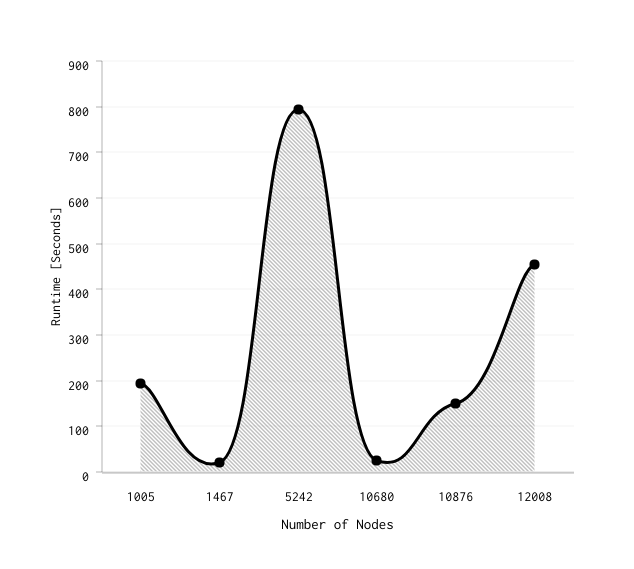
\includegraphics[width=\textwidth]{cnm-NodesVsRuntime}
    \caption*{(a)}
  \end{minipage}
  %\hfill
  \begin{minipage}[b]{0.4\textwidth}
    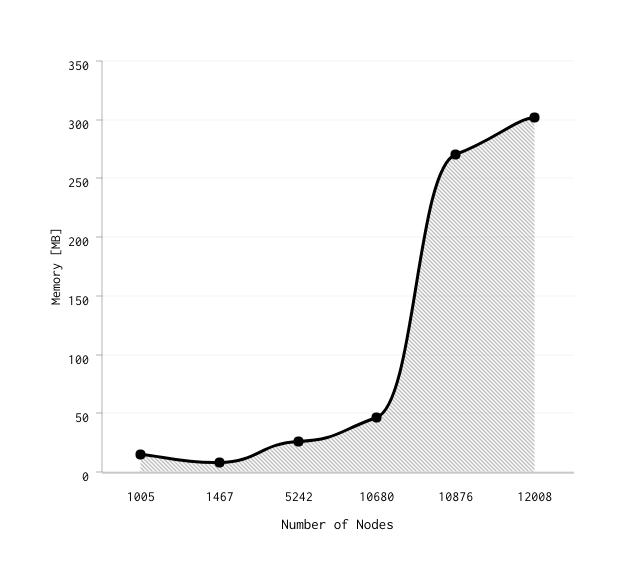
\includegraphics[width=\textwidth]{cnm-NodesVsMemory}
    \caption*{(b)}
  \end{minipage}
%\end{figure}
%
%% Plot run-time and memory against edges
%\begin{figure}[!tbp]
%  \centering
  \begin{minipage}[b]{0.4\textwidth}
    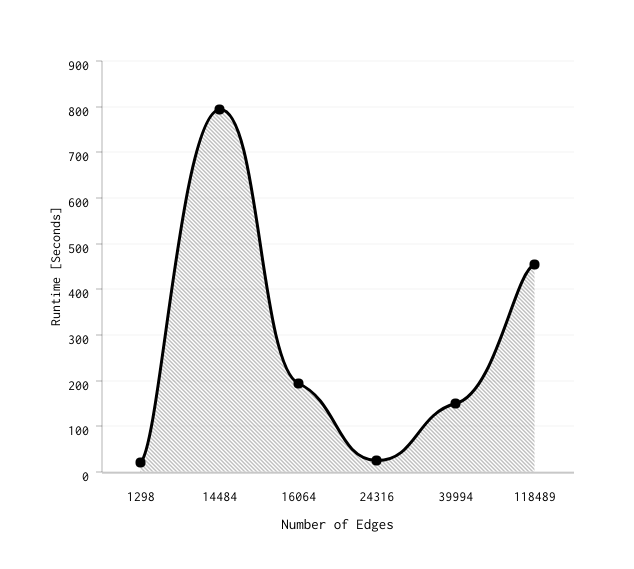
\includegraphics[width=\textwidth]{cnm-EdgesVsRuntime}
    \caption*{(c)}
  \end{minipage}
  %\hfill
  \begin{minipage}[b]{0.4\textwidth}
    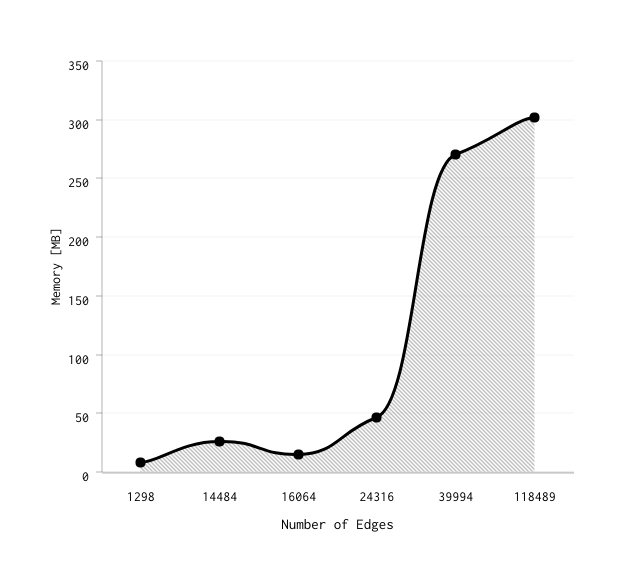
\includegraphics[width=\textwidth]{cnm-EdgesVsMemory}
    \caption*{(d)}
  \end{minipage}
%\end{figure}
%
%% Plot detected communities
%\begin{figure}[!tbp]
%  \centering
  \begin{minipage}[b]{0.4\textwidth}
    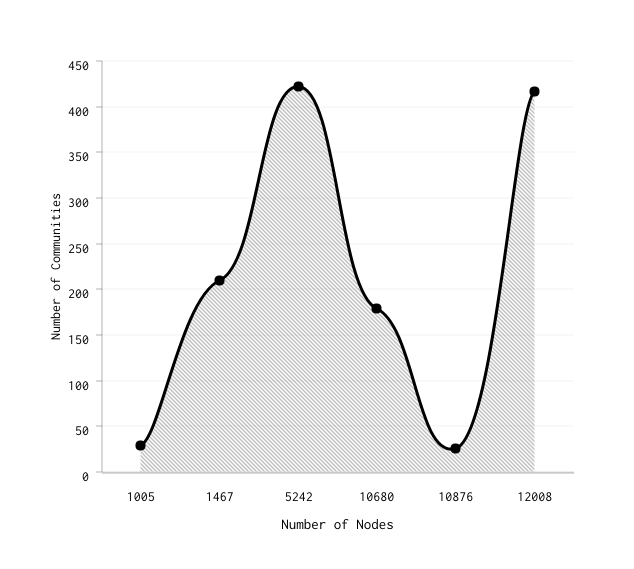
\includegraphics[width=\textwidth]{cnm-NodesVsCommunities}
    \caption*{(e)}
  \end{minipage}
  %\hfill
  \begin{minipage}[b]{0.4\textwidth}
    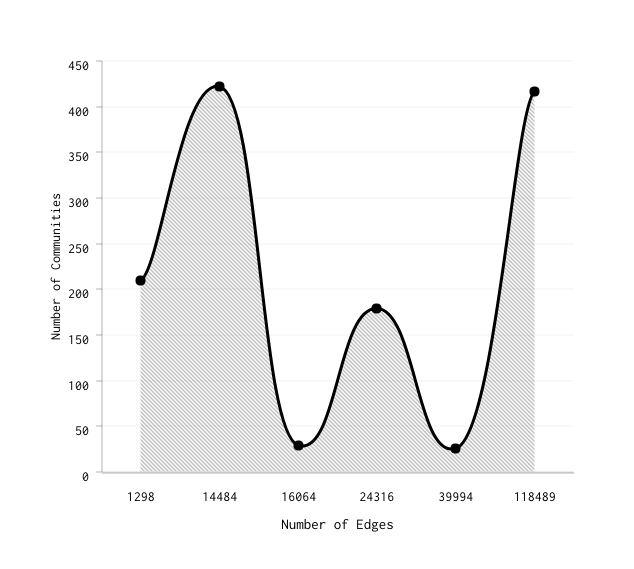
\includegraphics[width=\textwidth]{cnm-EdgesVsCommunities}
    \caption*{(f)}
  \end{minipage}
  \caption{Clauset-Newman-Moore algorithm: (a) run-time against number of nodes (b) Memory usage against number of nodes (c) run-time against number of edges (d) Memory usage against number of edges (e) Number of communities against number of nodes (f) Number of communities against number of edges}
  \label{fig:CNM-runs}
\end{figure}

\vfill
\pagebreak

\section{Algorithm Comparison}
In (\ref{sec:evaluation}), the algorithms and their performance on detecting community structure is discussed with the help of blockchain data. Clauset-Newman-Moore algorithm could not deliver on the run-time and memory consumption for blockchain data as expected. On the other hand Infomap algorithm and Louvain method algorithm seems promising for detecting community structures in blockchain transactions. So in this section, Clauset-Newman-Moore algorithm has been excluded from comparison.

Although both the algorithms (Infomap and Louvain method) had been discussed in details, in this section a comparison of run-time and memory consumption is drawn to better understand these two algorithms' performance on blockchain data-sets.

\begin{figure}[H]
  \centering
  \begin{minipage}[b]{0.4\textwidth}
    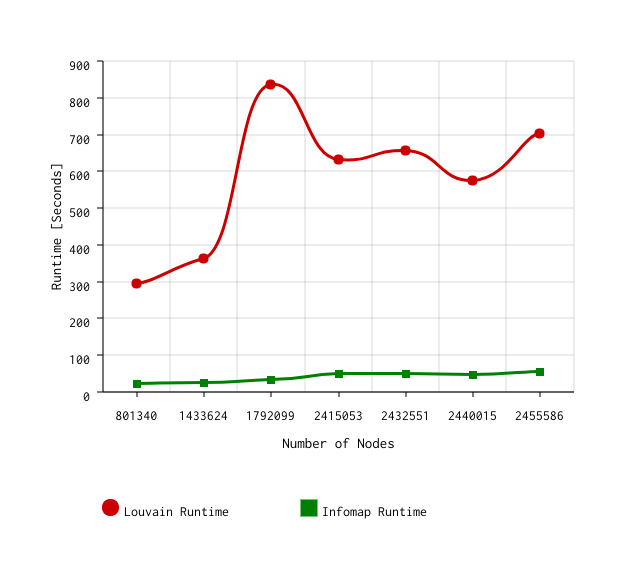
\includegraphics[width=\textwidth]{Mixed-NodesVsRuntime}
    \caption*{(a)}
  \end{minipage}
  %\hfill
  \begin{minipage}[b]{0.4\textwidth}
    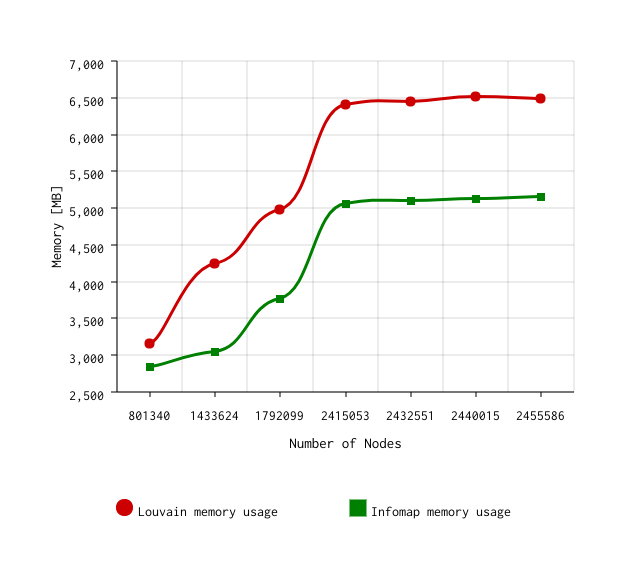
\includegraphics[width=\textwidth]{Mixed-NodesVsMemory}
    \caption*{(b)}
  \end{minipage}
  \begin{minipage}[b]{0.4\textwidth}
    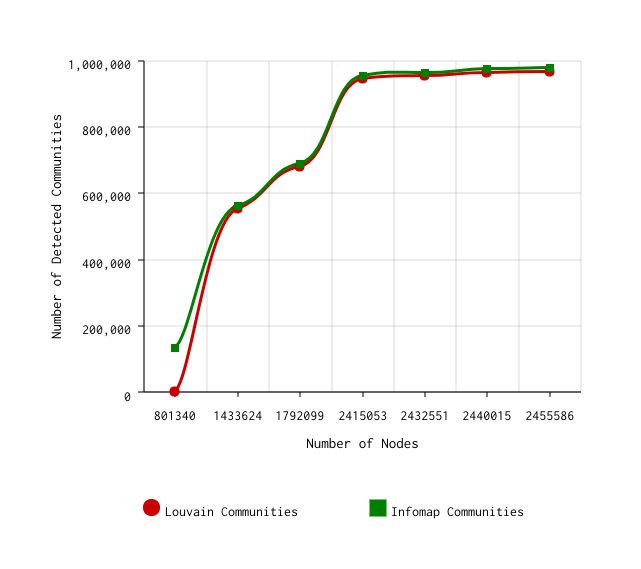
\includegraphics[width=\textwidth]{Mixed-NodesVsCommunities}
    \caption*{(c)}
  \end{minipage}
  \caption{Algorithm comparison: (a) run-time against number of nodes (b) Memory usage against number of nodes (c) Detected communities against number of nodes}
  \label{fig:algo-run-comparision}
\end{figure}

Figure (\ref{fig:algo-run-comparision}) (a), shows the run-time for both Infomap and Louvain method algorithm in respect to same amount of nodes from blockchain data-set. Same data set has been used to measure the run-time in both the algorithms. In (a), Infomap algorithm runs in less than a minute for 2.4 million nodes where Louvain method runs in a little over 11 minutes. In (b), Infomap algorithm costs 5.1 GB of RAM for 2.4 million nodes where Louvain method costs 6.4 GB for the same amount of nodes from the same blockchain data-set.

Figure (\ref{fig:algo-run-comparision}) (c), shows the amount of communities detected by Infomap and Louvain method algorithm from the same blockchain data-sets. Figure (c) reveals that although the first iteration of community detection gives two very different sets of results but both the algorithm detects nearly the same number of communities while the number of nodes keep increasing. Performance of both algorithms will increase with the increase of processing power and memory of the system used to run the algorithms.

\section{Evaluation of Observation Framework}
The proposed observation framework used blockchain data with three different algorithms and it's performance has been evaluated so far for the detection of communities. In chapter (\ref{cha:3_concept_and_design}) section (\ref{sec:framework}) the frame work creates sub graph of the previous graph's snapshot and merges all the nodes and edges with the current snapshot of data only if the node is present in top $n$ communities in the first graph snapshot. So after the merge, communities are detected and top $n$ communities are selected from the current (t+1) time-stamp data. A similarity measure described in chapter (\ref{cha:2_relatedwork}) is used to find the most similar community pairs to observe the changes in the community.

In Figure (\ref{fig:community_evolution_evaluation})(a) shows a single community structure from the Ehereum data of July, 2017 detected by the prototypical framework. This figure represent a single cluster of nodes that has been detect by the proposed framework. From the figure, it is observable that two nodes play very vital role in this community. Although the community detection algorithm detected all the nodes as one community, the figure is showing different clusters because of the layout algorithm used to visualize the underlying data. To visually observe changes in this community the visual layout will help.

Figure (\ref{fig:community_evolution_evaluation})(b) represents the community  from figure (a) in the next time-stamp, in this case, the community at next month (August, 2017). Figure (b) show the changes that happened to the previous community time interval of (t+1-t)= 1 time-stamp. It is observable that, community structure has changed in this time-stamp. The same nodes from previous time stamp was involved in more Ethereum transactions and that lead the network to create current community structure at time-stamp $t+1$.

Like figure (a) and (b), its noticeable that figure (c), (d) and (e), (f) shows the same properties of gaining more transactions and as result the community grew in size in each case. In Figure (\ref{fig:community_evolution_evaluation}), each pair of figures represents a community in two different time stamp and it's visible from the figures that all the pairs shows that the community is growing. This phenomenon is observed because of the popularity of ethereum blockchain cryptocurrency. Community could lose nodes, split into two and get merged with another community as described in section (\ref{sec:dynamic_community_algorithms}). The figures shown in this section of the thesis are only a visualization of three communities at two different timestamps. With the help of proposed prototypical framework it's possible to detect and observe communities as the evolve over time.

\begin{figure}[H]
  \centering
  \begin{minipage}[b]{0.4\textwidth}
    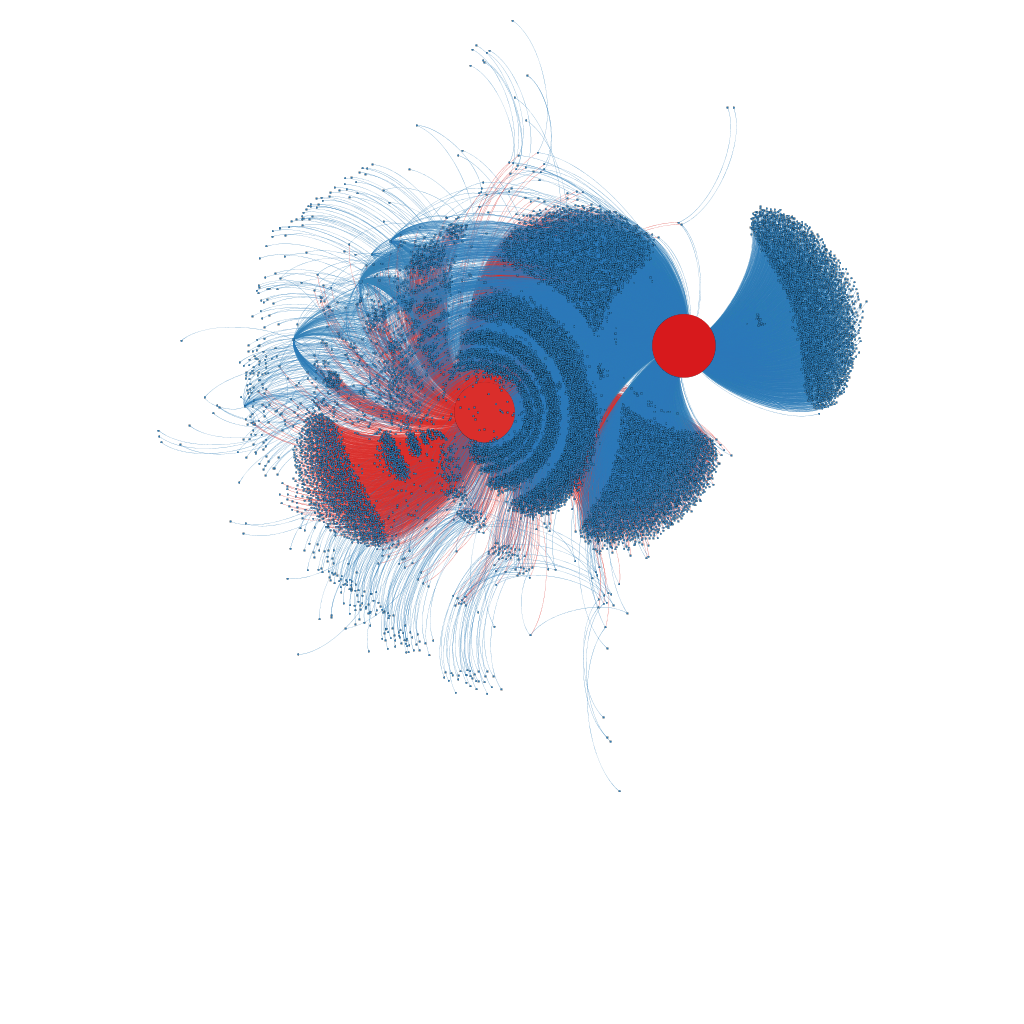
\includegraphics[width=\textwidth]{eos_community_t_1_2}
    \caption*{(a) snapshot at time $t$}
  \end{minipage}
  %\hfill
  \begin{minipage}[b]{0.4\textwidth}
    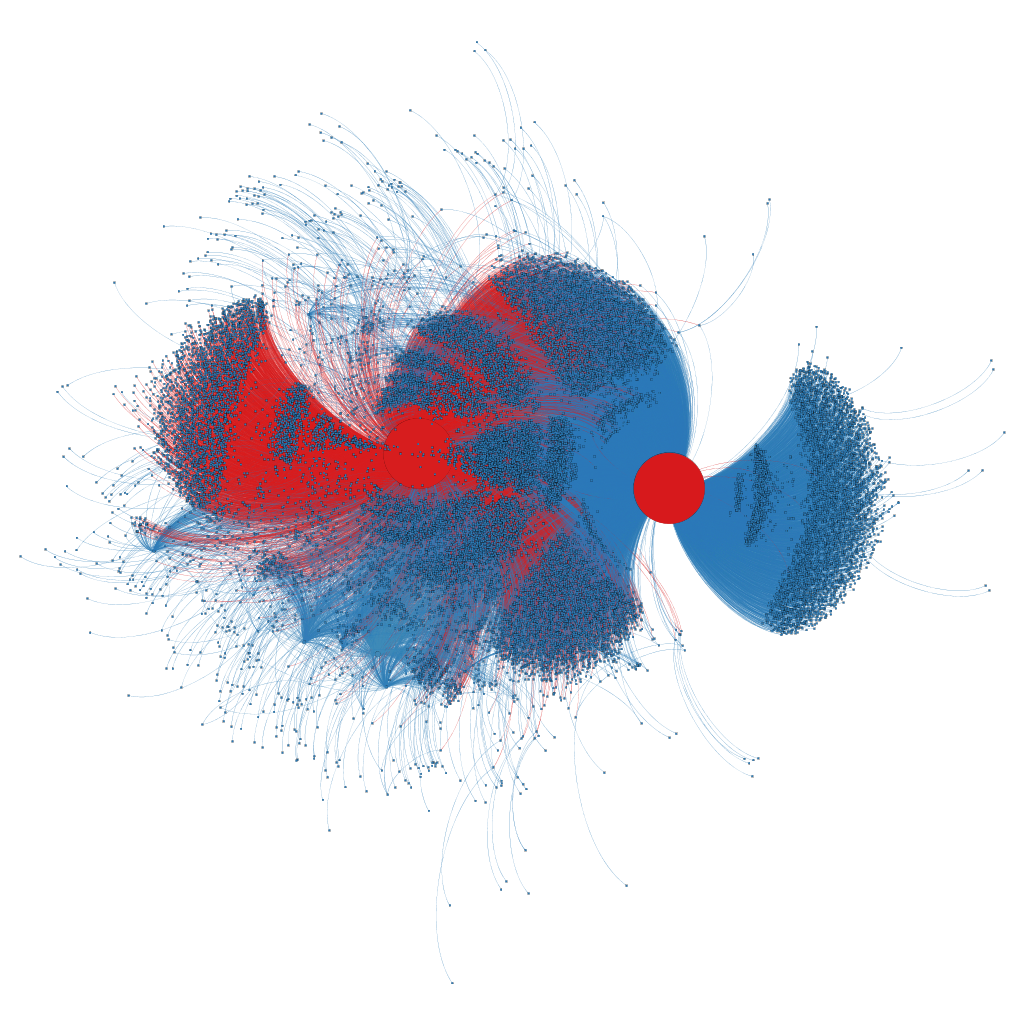
\includegraphics[width=\textwidth]{eos_community_t1_1_2}
    \caption*{(b) snapshot at time $t+1$}
  \end{minipage}
  \begin{minipage}[b]{0.4\textwidth}
    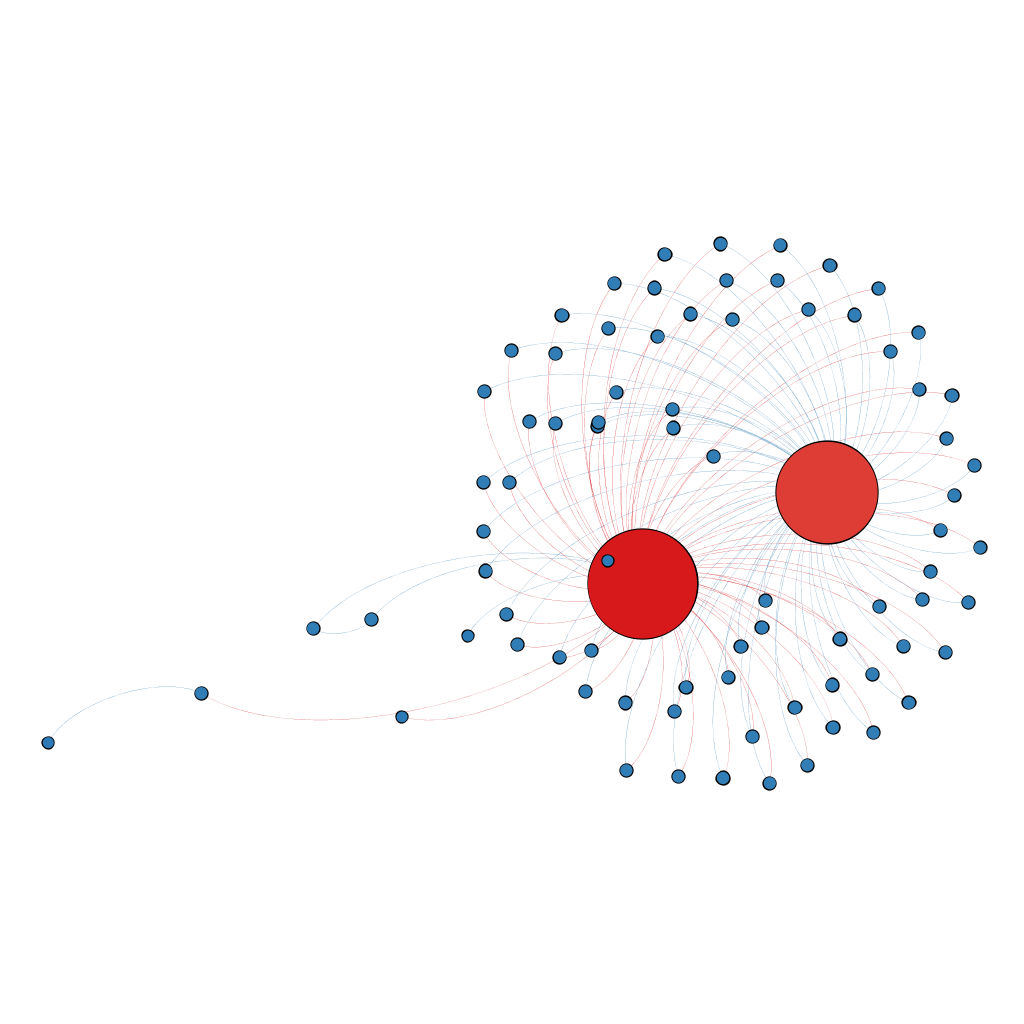
\includegraphics[width=\textwidth]{eos_community_t_15_24}
    \caption*{(c) snapshot at time $t$}
  \end{minipage}
  %\hfill
  \begin{minipage}[b]{0.4\textwidth}
    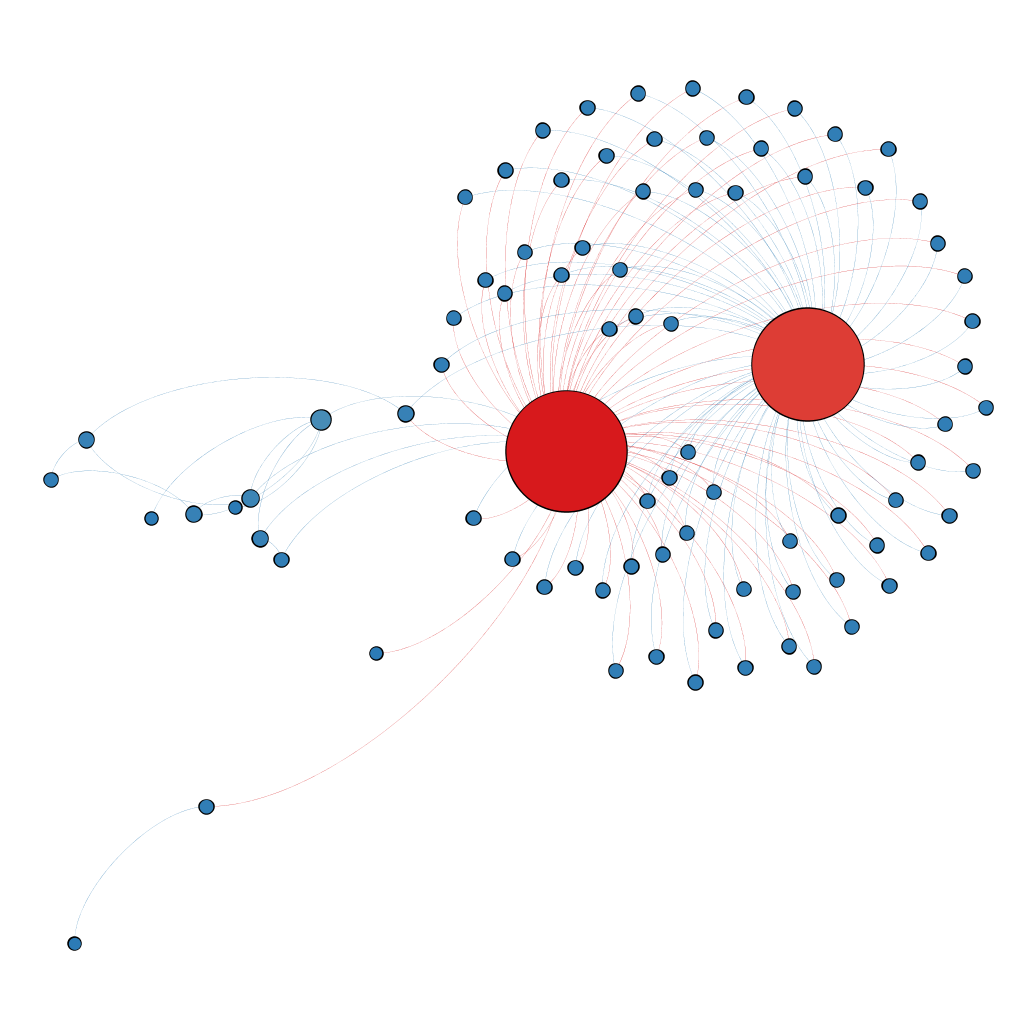
\includegraphics[width=\textwidth]{eos_community_t1_15_24}
    \caption*{(d) snapshot at time $t+1$}
  \end{minipage}
  \begin{minipage}[b]{0.4\textwidth}
    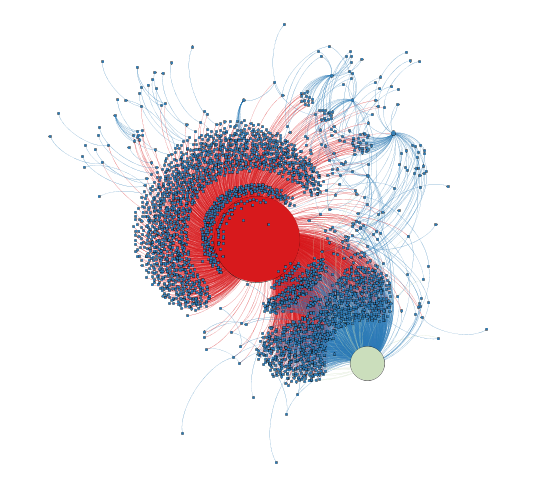
\includegraphics[width=\textwidth]{eos_community_t_6_8}
    \caption*{(e) snapshot at time $t$}
  \end{minipage}
  %\hfill
  \begin{minipage}[b]{0.4\textwidth}
    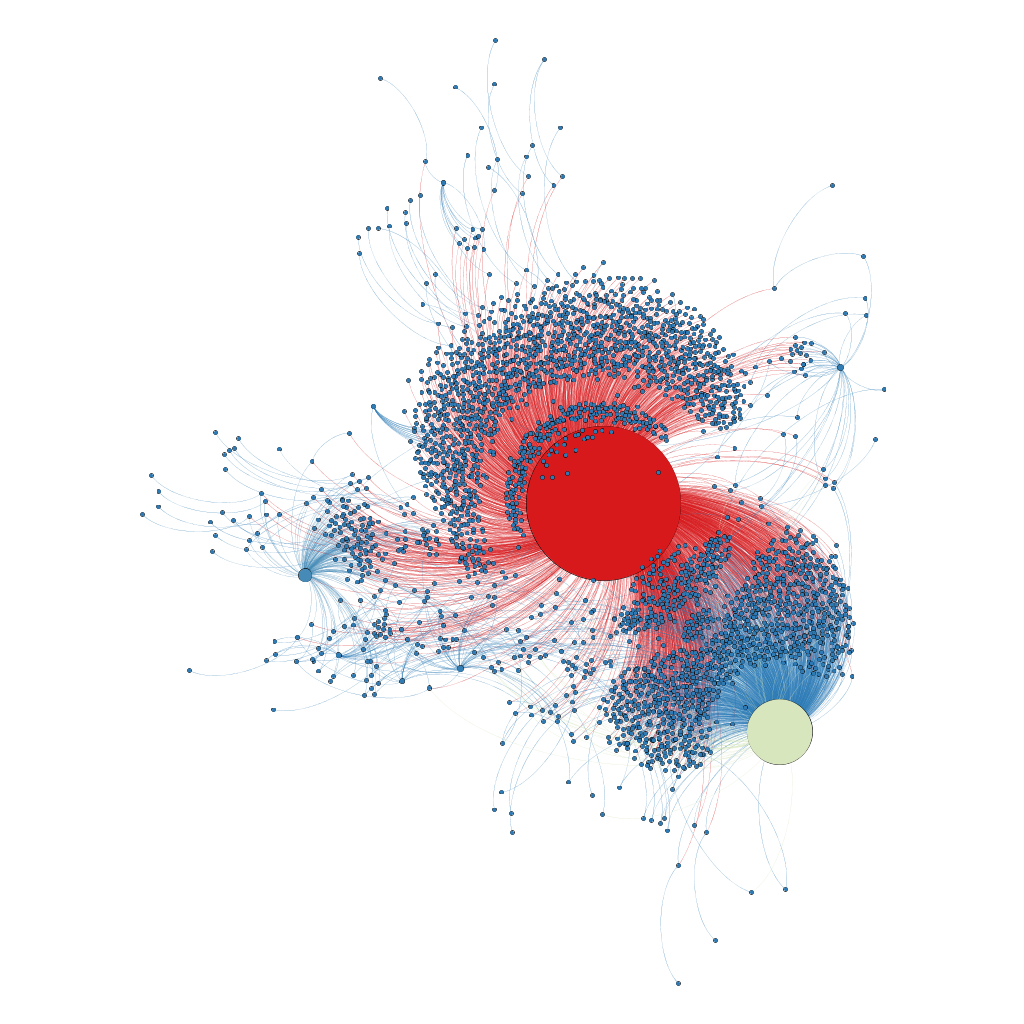
\includegraphics[width=\textwidth]{eos_community_t1_6_8}
    \caption*{(f) snapshot at time $t+1$}
  \end{minipage}
  \caption{Community evolution}
  \label{fig:community_evolution_evaluation}
\end{figure}
